% !TEX root=/home/tavant/these/manuscript/src/manuscript.tex

\section{Modeling the dielectric layer }
  \label{sec-diel_layer}
  
  The first effect of the wall material studied is effect of adding a layer of dielectric material with its own permittivity, as introduced in \Cref{sec-diel}.
  The simulation parameters are the same as in the canonical case, presented in \cref{sec-canonical}, but the plasma is separated from the ground wall by a dielectric layer of 3~cm.
  Hence, the distance between the grounded electrodes is $2.6\,\milli\meter$.
  The relative permittivity of the dielectric is $\epsr=25$.
  %% SEE runs 250et 257 ?? Ly=1cm, Diel avec et sans SEE
  
  \Cref{fig-diel_radial_Er} shows the radial profile of the radial electric field $E_R$ at $t=10\,\micro\second$ average in the azimuthal direction.
  The plasma domain starts at $r=0$ and finishes at $r=2\,\centi\meter$.
  We note the jump in the value of the electric field at the plasma-wall transition.
  This jump is due to the surface charges.
  We can also notice that in the dielectric layer, in $r < 0$ and $r > 2\,\centi\meter$, the radial electric field is close to zero, compared to the value in the sheath.
  
  \begin{figure}[hbtp]
    \centering
    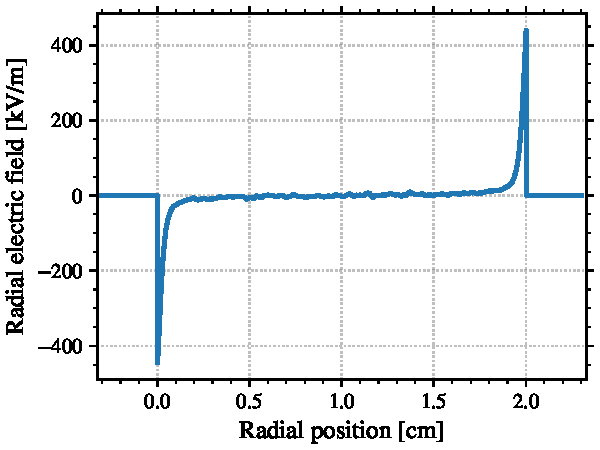
\includegraphics[width=\defaultwidth]{diel_average_radial_electric_field}
    \caption{Radial profile of the radial electric field $E_R$ average in the azimuthal direction at $t=10\,\micro\second$. The plasma domain starts at $r=0$ and finishes at $r=2\,\centi\meter$. The dielectric length is $L_{\\rm Diel} = 3\,\milli\meter$.  }
    \label{fig-diel_radial_Er}
  \end{figure}
  
  The next sections investigate the impact of the dielectric layer on the plasma characteristics, and highlight the plasma-wall interaction.
  
  \subsection{Effect of the dielectric layer} \label{subsec-effect_mob}
    
  
  The simulation results are qualitatively the same as in the case without the dielectric layer.
  As an example, \Cref{fig-mod_diel_comp} shows the temporal evolution of the axial electron mobility with and without the dielectric layer.
  We can see a small difference, but not really significant concerning the physical origin of the electron enhanced mobility, and the effect of the dielectric layer.
  The other variables (mean electron temperature, radial profiles, and so on) follow the same conclusion.
  
  \begin{figure}[hbtp]
    \centering
    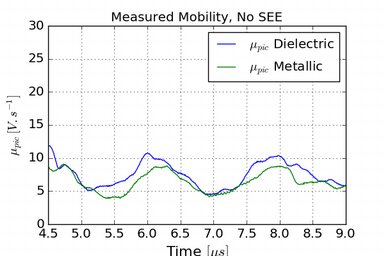
\includegraphics[width=\defaultwidth]{diel_mob_vs_time}
    \caption{Temporal evolution of the axial electron mobility with the dielectric layer and without (ground walls).}
    \label{fig-mod_diel_comp}
  \end{figure}
  \inlinenote{ Waiting for the rerun of the cases !!}
  
  \subsection{Near-wall parameters} \label{subsec-nearwall}
    In this section, we focus on the surface charge and the near-wall electric field.
    \Cref{fig-sigma_time} shows the temporal evolution of the surface charge at one point of the wall.
    The position has been chosen to be the center ($L_{\theta} = 0.25$~cm) of the lower wall, but the observations are similar at other positions.
     
    \begin{figure}[hbtp]
      \centering
      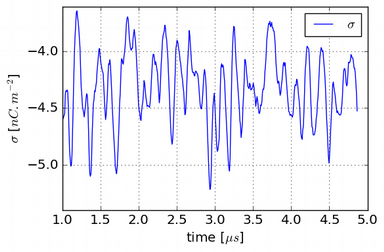
\includegraphics[width=\defaultwidth]{surface_charges_vstime}
      \caption{Temporal evolution of the surface charges at one position of the lower dielectric wall}
      \label{fig-sigma_time}
    \end{figure}
  
    \inlinenote{Anne: evolution temporelle de 1 a 5...pas clair pourquoi tu montres pas avant et apres...}
    
    We can see on \cref{fig-sigma_time} that the surface charge oscillates around a mean value close to $-4.5$ nC/\square\meter and an amplitude of around 1 nC/\square\meter.
    
    \inlinenote{Est-ce qu'on compare la valeur moyenne à la valeur theo d'un model de gain ? Ajouter quelque chose dans cette partie ?}
    
    
  \subsection{Dielectric model comparison} \label{subsec-modelcomp}
  
  \inlinenote{Anne: {\bf Beaucoup de remarques sur cette partie: pas assez claire, décrire plus les valeures observées, etc. Voir les notes sur le pdf (22 juillet)}}
  
  As introduced in \cref{sec-diel}, a simplified approach to model the effect of the surface charges on the plasma is to use a Neumann boundary condition [{\bf REF}]
  \begin{equation} \label{eq-neuman}
    E_r = \frac{\sigma}{\epsilon_0}.
  \end{equation}
  \Cref{eq-neuman} uses two approximations\string:
  \begin{itemize}
    \item one dimensional
    \item No electric field in the dielectric
  \end{itemize}
  
  \Cref{fig-er_time} shows the radial electric field inside of the dielectric and compare the electric field at the wall and compares it to \cref{eq-neuman}.
  
  \renewcommand\subfigurewidth{0.45\textwidth}

  \begin{figure}[hbtp]
    \centering
    \begin{tabular}{c c}
      \subfigure{electric_field_vstime}{a}{10, 20}
          &
      \subfigure{comp_sigma_Er_vstime}{b}{10, 20}
    \end{tabular}
    \caption{Temporal evolution of ({\bf a}) the radial electric field near the wall at the same azimuthal position than \cref{fig-sigma_time}, and ({\bf b}) the comparison with the near-wall electric field and  \cref{eq-neuman}, using the surface charge of \cref{fig-sigma_time}. }
    \label{fig-er_time}
  \end{figure}
  
  We can see on \cref{fig-er_time}.{\bf a} that the electric field in the wall in not zero, but oscillates around a value close to zero ($\sim 100$~V/m).
  Its amplitude is of the order of $4$~kV/m.
  
  \Cref{fig-er_time}.{\bf b} shows the near-wall  radial electric field compared to \cref{eq-neuman} at the same position than \cref{fig-sigma_time}.
  We can see that the two values are of the same order of magnitude, close to $-500$~kV/m.
  However, the two values are not strictly equal, but the maximum error between the two are only of the order of $20\%$, which mean that the \ac{RMS} error is around 10\%.
  
  \inlinenote{Anne: Small conclusion needed here. maybe conclude that this difference on electric field could have an influence on surface processes + not so difficult to include dielectric + 2D effects could be modeled more accurately Also you use it in the section 2.6 so you could already mention it here...In this section, no secondary electron has been taken into account, in section 2.6, we will also disuss the influence of using the simplified equation 2.8 in the case where secondary electron emission is important.}